% ============================================================================
%  DNU Lab Research Report --- DRAFT
%  "Generalization of Algorithmic Tasks in Micro-LLMs"
%  John Lee, Dickinson College. Advisor: Prof. John MacCormick.
%
%  FORMAT: NeurIPS 2026 main-track style (max 9 content pages; references,
%  appendices, and the Use-of-AI section do NOT count toward the limit).
%
%  HOW TO COMPILE (Overleaf, local = source of truth):
%   - Uses the NeurIPS 2026 style: neurips_2026.sty must be in the Overleaf
%     project (uploaded from the template). Also upload references.bib and the
%     two figure PNGs, then Recompile.
%   - Workflow: edit locally in report/, then copy main.tex into the Overleaf
%     project (and re-upload references.bib / figures whenever they change).
% ============================================================================

\documentclass{article}

% ---- NeurIPS 2026 style (neurips_2026.sty must be in the Overleaf project).
%      'preprint' shows author names (not anonymized); this is a DNU Lab report,
%      not a blind submission. The style loads natbib itself, so do not also
%      \usepackage{natbib} or \usepackage{geometry} here.
\usepackage[preprint]{neurips_2026}

\usepackage[utf8]{inputenc}
\usepackage[T1]{fontenc}
\usepackage{hyperref}
\usepackage{url}
\usepackage{booktabs}
\usepackage{amsmath}
\usepackage{graphicx}
\usepackage{xcolor}

% figures: kept in this folder (report/) so the same path works locally and on
% Overleaf (upload the two PNGs to the project root). Originals live in
% ../generalization-order/log/figures/ ; re-copy them here after regenerating.
\graphicspath{{.}{./figures/}}

% small helper for author notes still to be resolved (delete before submitting)
\newcommand{\todo}[1]{\textcolor{red}{[TODO: #1]}}

\title{Relative vs.\ Absolute Positional Encoding Predicts
Fixed-Length Position Generalization in Micro-Transformers}

\author{%
  John Lee \\
  Department of Computer Science \\
  Dickinson College \\
  \texttt{leejo@dickinson.edu} \\
}

\begin{document}

\maketitle

% ============================================================================
\begin{abstract}
% [Write this LAST. ~150--200 words. Should be understandable on its own.]
Length generalization, training on short sequences and testing on longer ones,
has been studied extensively. But a transformer can also fail without any change
in sequence length: the shift can be over \emph{where} a task-relevant symbol
sits within a fixed length. We study this fixed-length, held-out-position setting
on a micro-transformer (under one million parameters), trained from scratch to
decide which of two marked symbols in a string comes first. We train with both
symbols in the first half of the string and test with both in the second half, and
we compare five positional encodings under an otherwise identical model. All five learn the trained
positions perfectly, but only the relative encodings (no positional encoding,
rotary, and a T5-style relative bias) generalize to the held-out positions,
while the absolute encodings (learned and sinusoidal) do not transfer reliably.
The relative/absolute distinction, not the individual method, predicts
which encodings generalize. Notably, rotary encoding (reported to generalize
poorly for length) generalizes here, landing with the relative encodings,
suggesting that generalization over position at fixed length is a distinct
phenomenon from length generalization.
\end{abstract}

% ============================================================================
\section{Introduction}
% [Write this LAST. ~700 words. At minimum, expand the abstract; add motivation
%  and preview the main results.]

Transformers often fail to generalize beyond the sequences they were trained on,
and much of the work on this failure has focused on \emph{length}: a model
trained on short inputs is tested on longer ones, and the test positions are ones
the model never saw during training. But length is not the only axis along which
the input distribution can shift. Consider a task defined on a fixed-length
input, where the answer depends on \emph{where} a special symbol sits. We can
train only on examples where the symbol falls in the first half of the input,
then test on examples where it falls in the second half, all without changing
the length. Every position is present in every example; what the model has not
seen is the symbol placed at the held-out positions. This is a distribution shift over
position within a fixed length, not over length.

This report asks whether a micro-transformer (under one million parameters)
generalizes across such a position shift, and whether the choice of positional
encoding decides the outcome. The setting is deliberately small. Most work on
transformer generalization uses models large enough to require substantial
compute. Models this small are comparatively understudied, and they can be trained
from scratch on an ordinary CPU. This keeps each experiment cheap, so we can run
many seeds and control every position exactly.

We study a relative-order task on a fixed-length string: given one \texttt{X} and
one \texttt{Y}, the model decides which comes first. To test generalization we
split the data by position, training with both symbols in the first half of the
string and testing with both in the second half. All five runs use the same
model; only the positional encoding differs. We compare three relative encodings
and two absolute ones. The three relative ones are no positional encoding (NoPE),
rotary (RoPE), and a T5-style relative bias (T5); the two absolute ones are a
learned positional encoding and a sinusoidal positional encoding.

Our main finding is a separation by family. All five encodings fit the trained
positions perfectly, so the task is learnable in every case. On the held-out
positions, the three relative encodings generalize, averaging 95.7\% to 99.2\%.
The two absolute encodings do not. Sinusoidal stays below chance, and learned
lands near 69\% on average but is highly variable across seeds. The
distinction that predicts generalization is not the specific method but the family,
whether the encoding is relative or absolute. Within the absolute family, the two
encodings even fail differently, which we revisit in the analysis.

Our contributions are: (i) a fixed-length, position-split evaluation that
isolates position generalization from length generalization; (ii) a five-way
comparison of positional encodings under this split on a micro-transformer; and
(iii) the finding that the relative/absolute distinction predicts which encodings
generalize, and that this setting is distinct from length generalization: most
visibly, rotary encoding fails there but succeeds here.

% ============================================================================
\section{Related Work}
% [~400 words. REQUIRED. Describe the RELATIONSHIP to prior work, not a summary.]

This report describes the output of an independent research project in the DNU
Lab of Dickinson College. By design, DNU Lab projects focus on conducting
research rather than surveying existing work. In this section we describe only
one piece of related work. This serves as an initial step toward a more complete
literature survey.

The closest prior work is \citet{kazemnejad2023impact}, who compare positional
encodings for length generalization in decoder-only transformers. Their study
spans ten tasks and models of around 100M parameters. They train on
short sequences and test on longer ones, so the test positions never appear
during training. They report that NoPE generalizes best, followed by the T5 bias,
with the absolute encodings among the worst. We study the same underlying question, but over a different axis. Does the choice
of positional encoding decide whether a model generalizes to unseen situations? Our input
length is fixed, so every position is seen during training; the shift is over the
\emph{placement} of the task-relevant symbols, not over length.

The relationship is threefold. First, our result partly \emph{reproduces} theirs:
the relative encodings (NoPE and the T5-style bias) generalize while the absolute
encodings fail, as in their setting.
Second, our setting \emph{complements} theirs by testing what they cannot. They
can only evaluate a sinusoidal absolute encoding, because a learned one has no
parameters for positions never seen in training. Our fixed-length setting exposes
every position, so we can evaluate a learned absolute encoding directly. Third, and most tellingly, the two settings
\emph{diverge} on RoPE. \citet{kazemnejad2023impact} report that it generalizes
poorly and behaves much like an absolute encoding. In our fixed-length setting,
RoPE instead lands firmly on the relative side (95.7\% on average, far above
either absolute encoding). The same method landing on
opposite sides of the relative/absolute divide suggests that length generalization
and fixed-length position generalization are not the same phenomenon.

% ============================================================================
\section{Experimental Design}
% [~1100 words. The conceptual core (the position split) lives here.]

\subsection{Task}
Each input is a length-20 string made of the digits \texttt{0}--\texttt{9} with
exactly one \texttt{X} and one \texttt{Y} substituted in, followed by a
separator \texttt{:} and a single answer token. The label is \texttt{T} if the
index of \texttt{X} is smaller than the index of \texttt{Y}, and \texttt{F}
otherwise. The other eighteen characters are random digits and do not affect the
label. Two examples:

\begin{center}
\begin{tabular}{ll}
\texttt{X904Y482520615370751:T} & (\texttt{X} at 0, \texttt{Y} at 4 $\rightarrow$ \texttt{T}) \\
\texttt{5337854YX80803953079:F} & (\texttt{Y} at 7, \texttt{X} at 8 $\rightarrow$ \texttt{F}) \\
\end{tabular}
\end{center}

\noindent The model reads the string and the separator and predicts one token.
Because the answer is a single token, chance accuracy is 50\%, and we keep the
two classes balanced so that accuracy is meaningful. The model's input vocabulary
is the ten digits, \texttt{X}, \texttt{Y}, and the separator \texttt{:}; the two
labels \texttt{T} and \texttt{F} appear only as the output token.

\subsection{The position split}
The generalization test is created entirely by controlling \emph{where}
\texttt{X} and \texttt{Y} are allowed to appear. This report uses the \texttt{half} split
throughout: training and validation examples place both symbols in the first half
of the string (indices 0--9), while the held-out test examples place both in the
second half (indices 10--19). The input
length is 20 in every pool, so the model sees all 20 positions in every example;
the only thing withheld from training is the configuration in which the symbols
occupy the second half.

We generate three separate pools rather than slicing one
stream. The training and validation pools both use the first-half positions;
validation holds unseen examples for monitoring only. The generalization test pool uses the
held-out positions and is never seen during training. The pools hold 50{,}000
training, 5{,}000 validation, and 2{,}000 test examples, each balanced 50/50
between \texttt{T} and \texttt{F}.

This design isolates position generalization from length generalization. The
input never changes length, so any gap between validation and test accuracy is a
failure to transfer a rule from trained positions to held-out positions, not a
failure to extrapolate to unseen positions.

\subsection{Model and training}
All runs use the same decoder-only transformer implemented from scratch, with
four layers, four attention heads, and an embedding width of 128, for
approximately 0.8M parameters and a causal attention mask. Each example is 22
tokens long, well within the context length of 64. The only independent variable
across runs is the positional encoding. Training uses AdamW with learning rate $10^{-3}$ (decayed
to $10^{-4}$ with a 100-iteration warmup), batch size 64, for 2000 iterations on
CPU. The loss is computed only on the final answer token, not on the digits, so
the model is scored on the classification decision rather than on modeling the
input stream.

\subsection{The five positional encodings}
We compare three relative and two absolute encodings, holding the rest of the
architecture fixed:
\begin{itemize}
  \item \textbf{Relative.} \emph{No positional encoding} (NoPE): no position
  signal is added; order information is available only through the causal
  attention mask, which lets NoPE learn relative-position patterns
  \citep{kazemnejad2023impact}. \emph{RoPE}~\citep{su2021roformer}: query and key vectors are
  rotated by an angle proportional to their absolute position, so that the
  attention dot product depends only on the relative offset between tokens.
  \emph{T5-style relative bias}~\citep{raffel2020t5}: a learned scalar bias
  indexed by the relative distance between query and key is added to the attention
  score, using the standard T5 bucketing (exact buckets for nearby offsets and
  log-spaced buckets for far ones; 32 buckets, causal).
  \item \textbf{Absolute.} \emph{Learned}: a trainable position embedding is
  added to the token embedding at each index. \emph{Sinusoidal}: the fixed
  sine/cosine table of \citet{vaswani2017attention} is added instead.
\end{itemize}

\subsection{Seeds and reporting}
We run ten seeds per encoding. Each seed regenerates the data split, so a seed
varies the training and test examples as well as the model initialization and
batch order; the reported spread therefore reflects data-sampling variance, not
only initialization noise. We report accuracy on the in-distribution validation
pool (trained positions) and on the generalization test pool (held-out positions),
as the mean over seeds. We also give the per-seed breakdown, so the family
separation can be compared against seed variation.

% ============================================================================
\section{Results}
% [~900 words. Facts only; interpretation goes in Section 5.]

Table~\ref{tab:main} reports validation and held-out accuracy for each encoding,
as the mean and standard deviation over ten seeds. Every encoding reaches 100\%
validation accuracy, so all five learn the task on the trained positions. The encodings separate by family
on the held-out positions: the three relative encodings average between 95.7\% and
99.2\%, while the two absolute encodings average 68.6\% (learned) and 31.9\%
(sinusoidal), both well below the relative family. The relative/absolute gap
(roughly 27 to 67 percentage points) is far larger than the standard error of any
mean, so the separation is robust.

\begin{table}[t]
  \centering
  \caption{Accuracy on the \texttt{half} split, mean $\pm$ standard deviation over
  ten seeds (each seed regenerates the data split). Validation is on trained
  positions (0--9); held-out test is on positions 10--19. Chance is 50\%. All five
  encodings learn the task; the relative family generalizes while the absolute
  family does not.}
  \label{tab:main}
  \begin{tabular}{llcc}
    \toprule
    Encoding & Family & Val (trained pos.) & Held-out (unseen pos.) \\
    \midrule
    NoPE (causal mask) & relative & 100\% & $99.2 \pm 1.7$ \\
    T5 relative bias   & relative & 100\% & $99.2 \pm 2.1$ \\
    RoPE               & relative & 100\% & $95.7 \pm 6.8$ \\
    Learned            & absolute & 100\% & $68.6 \pm 18.1$ \\
    Sinusoidal         & absolute & 100\% & $31.9 \pm 6.9$ \\
    \bottomrule
  \end{tabular}
\end{table}

The per-seed breakdown (Table~\ref{tab:perseed}) shows that the family gap holds on
every seed, but also that the encodings differ in stability. The relative
encodings are consistently high; among them, RoPE is the least stable, dropping
to 79.6\% on one seed while NoPE and the T5 bias never fall below 92.9\%. The two
absolute encodings behave very differently from each other. Sinusoidal is
consistently below chance on every seed (19.2\% to 42.7\%). Learned is highly
variable: it ranges from 50.0\% (pure chance) up to 100\% on one seed, with two
further seeds above 89\%. The absolute family therefore does not fail uniformly:
one member fails robustly, the other fails only on average and occasionally
generalizes.

\begin{table}[t]
  \centering
  \caption{Held-out accuracy by seed on the \texttt{half} split (each seed's own
  data split). The relative family stays high on every seed; sinusoidal is
  consistently below chance; learned is highly variable (50\% to 100\%).}
  \label{tab:perseed}
  \begin{tabular}{lccccc}
    \toprule
    Seed & NoPE & RoPE & T5 & Learned & Sinusoidal \\
    \midrule
    1337 & 100.0 &  99.7 & 100.0 &  69.0 & 30.6 \\
    1338 &  97.5 &  92.8 & 100.0 &  50.0 & 26.4 \\
    1339 & 100.0 & 100.0 & 100.0 &  89.7 & 36.6 \\
    1340 & 100.0 & 100.0 & 100.0 &  69.1 & 40.6 \\
    1341 &  94.7 &  79.6 & 100.0 & 100.0 & 33.2 \\
    1342 & 100.0 & 100.0 &  92.9 &  50.0 & 35.4 \\
    1343 & 100.0 &  86.5 & 100.0 &  92.7 & 29.1 \\
    1344 & 100.0 &  98.3 &  99.3 &  60.0 & 42.7 \\
    1345 & 100.0 & 100.0 & 100.0 &  50.0 & 24.6 \\
    1346 & 100.0 & 100.0 & 100.0 &  55.6 & 19.2 \\
    \midrule
    Mean & 99.2 & 95.7 & 99.2 & 68.6 & 31.9 \\
    \bottomrule
  \end{tabular}
\end{table}

Figure~\ref{fig:heldout} plots held-out accuracy per encoding with the individual
seeds overlaid. Because every encoding reaches 100\% validation accuracy, each gap
below it is a failure to generalize, not a failure to learn.

\begin{figure}[t]
  \centering
  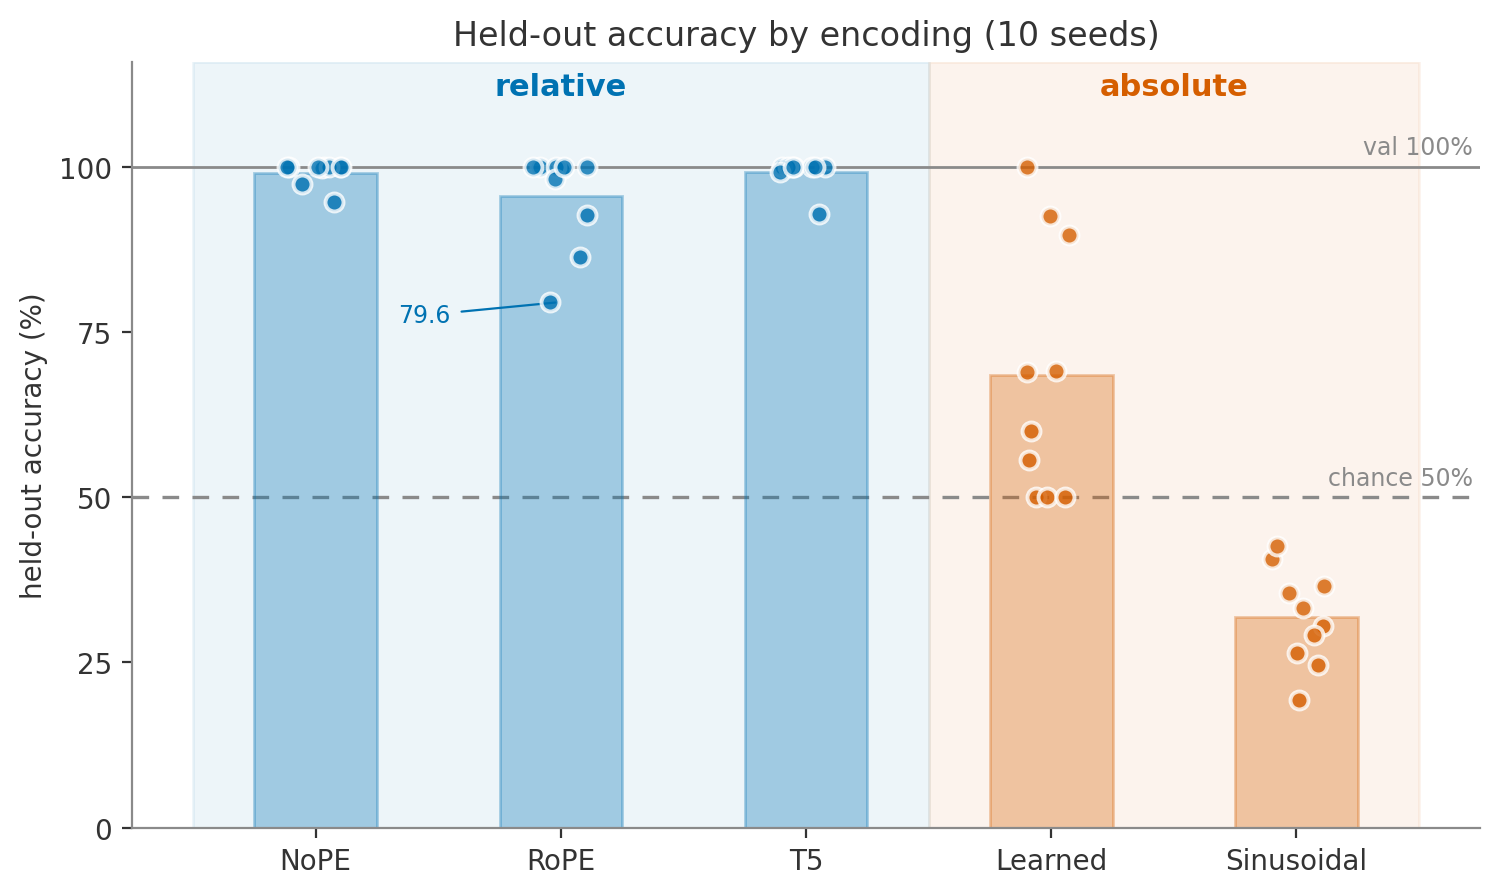
\includegraphics[width=0.9\textwidth]{heldout_bar_multiseed.png}
  \caption{Held-out accuracy by encoding on the \texttt{half} split. Bars are the
  mean over ten seeds; each dot is one seed (a box plot is misleading at $n=10$).
  The relative family sits near the val=100\% line; learned straddles chance with a
  wide, bimodal spread, so its mean bar (68.6\%) is a value no single seed produced;
  sinusoidal sits below chance. RoPE's one low seed (79.6\%) is labelled. Because
  every encoding reaches 100\% validation accuracy, each gap below it is a
  generalization failure, not a learning failure.}
  \label{fig:heldout}
\end{figure}

Figure~\ref{fig:perpos} breaks the same accuracy down by the positions of
\texttt{X} and \texttt{Y}. The relative encodings are correct across the whole
grid, while the absolute encodings are correct only in the trained block
(top-left) and break on the held-out positions (bottom-right), where learned is
uneven and sinusoidal falls well below chance.

\begin{figure}[t]
  \centering
  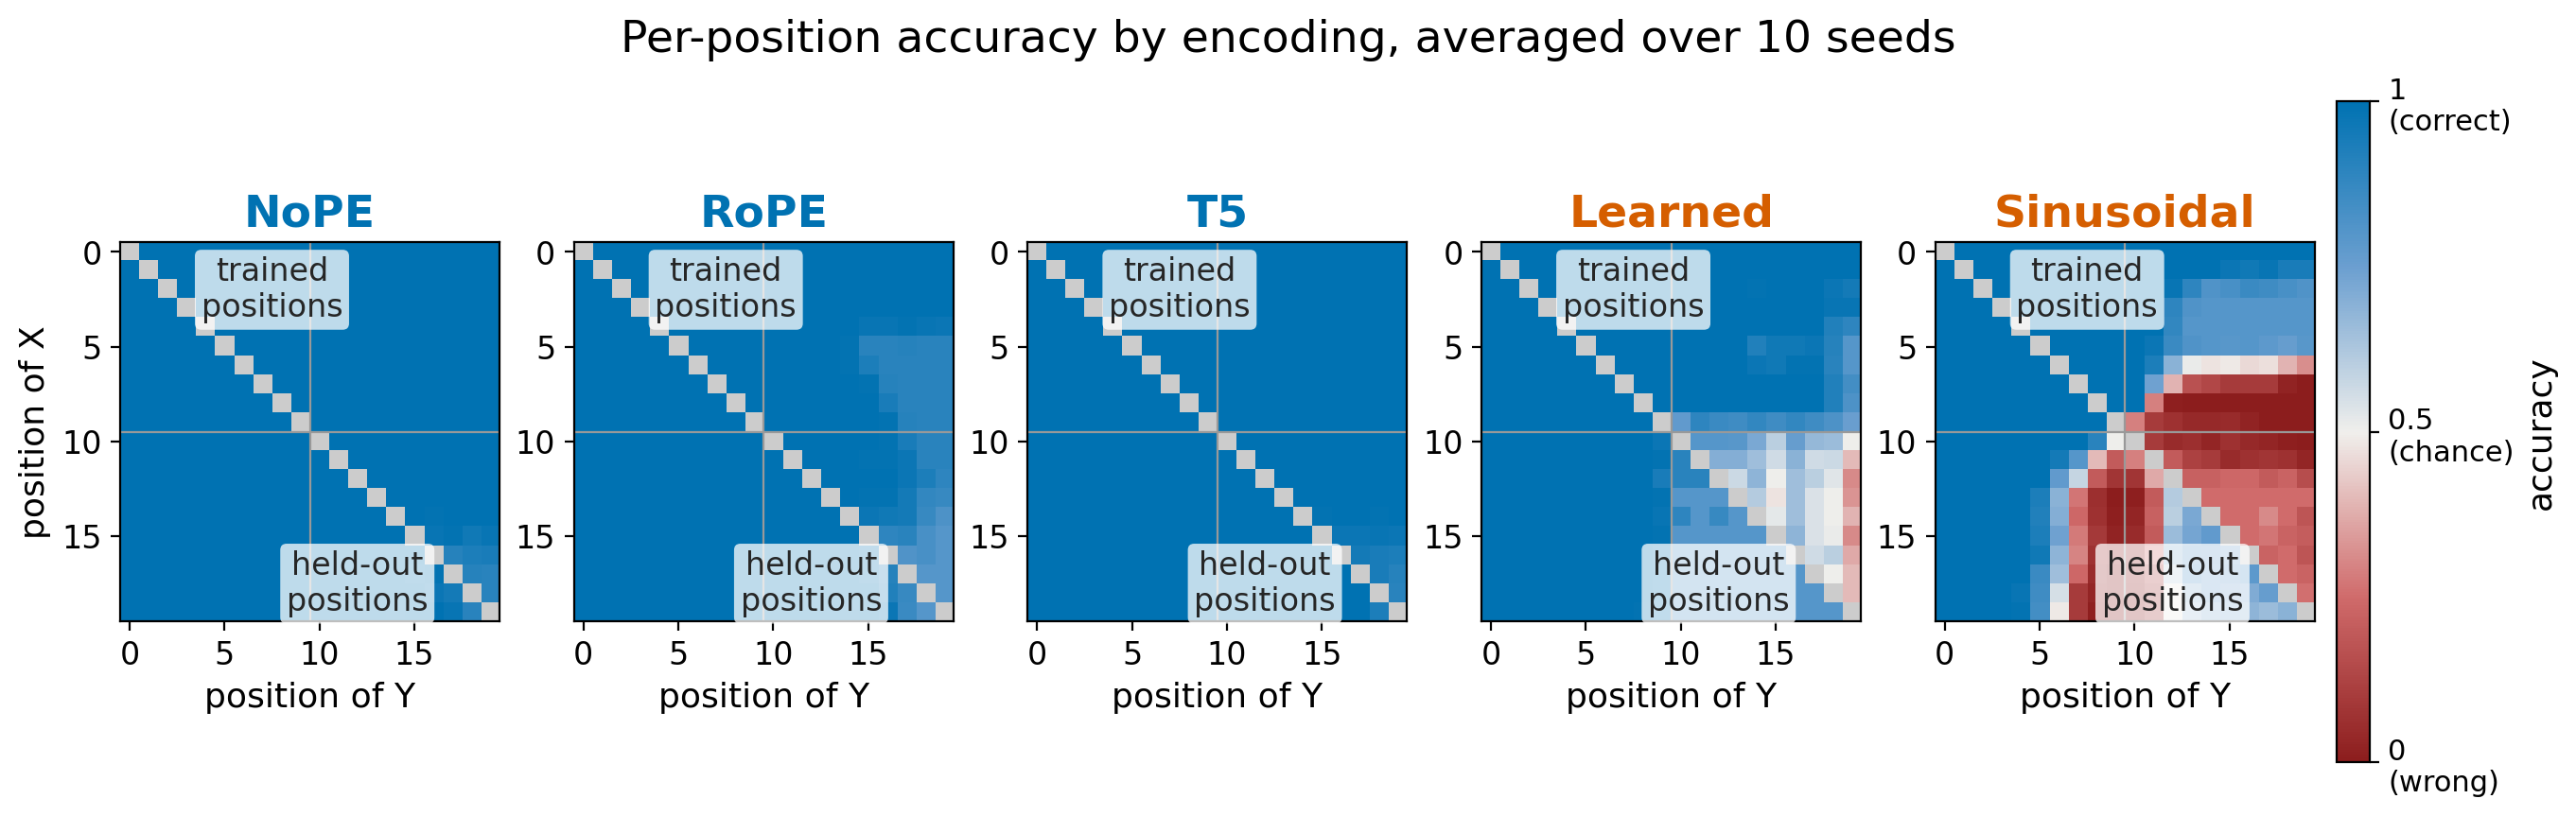
\includegraphics[width=\textwidth]{per_position_multiseed.png}
  \caption{Per-position accuracy by encoding, averaged over ten seeds. Cell =
  accuracy with \texttt{X} at the row position and \texttt{Y} at the column
  position; the grey diagonal ($x=y$) is excluded because the two symbols never
  share a cell. Relative encodings are correct everywhere; the absolute encodings
  are correct in the trained block and fail in the held-out block. Colour is a
  colour-blind-safe diverging map (blue = correct, grey = chance, red = below
  chance). Sinusoidal's red/blue triangular split in the held-out block reflects
  collapse to a single label, not distance reading.}
  \label{fig:perpos}
\end{figure}

% ============================================================================
\section{Analysis}
% [~800 words. Interpretation and honest limitations.]

\subsection{Why the relative encodings generalize}
The relative encodings express the answer through the offset between positions
rather than through the positions themselves. NoPE has order information only
through the causal mask, which reflects whether one token precedes another;
RoPE makes the attention dot product a function of the offset between two
tokens; the T5-style bias is indexed directly by relative distance. A rule stated
in terms of relative offset (is \texttt{X} before or after \texttt{Y}?) is the
same rule in the first half and the second half of the string, so a model that
learns it on the trained positions applies it unchanged on the held-out
positions. The absolute encodings tie the computation to the specific indices
seen in training (0--9). On the held-out indices (10--19) those features do not
carry the meaning the model learned, so the model misfires.

\subsection{Two ways for an absolute encoding to fail}
The two absolute encodings are both absolute, but they fail in different ways, and
the difference points to a mechanism. Sinusoidal fails robustly: it is below chance
on every seed ($31.9 \pm 6.9$), because its position vectors are fixed by a formula
and never adapt. The vectors for the held-out positions produce a definite signal,
but the rule the model attached to that signal in the first half is wrong in the
second half, so the model is confidently incorrect rather than merely guessing.
Learned fails on average but not reliably: it varies from pure chance to full
generalization across seeds ($68.6 \pm 18.1$, up to 100\% on one split). We
attribute this to how the two encodings treat the held-out positions during
training. In our fixed-length inputs every position is occupied in every example,
so the learned position embeddings for indices 10--19 do receive gradient
updates, from the filler digits that sit there, even though \texttt{X} and
\texttt{Y} never do. Whether those embeddings happen to develop features usable for
the order computation is init- and data-dependent, which produces the large seed
variance. Sinusoidal's held-out vectors, being fixed, never get this chance, which
is why it fails consistently. This asymmetry is invisible in a length-generalization
setting, where the held-out positions do not exist during training at all.

\subsection{Limitations}
Several limits should temper how far this result is read. The study covers a
single task, a single split, and a single fixed length, so we cannot yet say the
relative/absolute line holds across position-dependent tasks in general. The ten
seeds each regenerate the data split, so the reported spread reflects both
model-initialization and data-sampling variance; still, ten seeds pin down the
family separation far better than they pin down the learned encoding's mean, whose
large variance would need more seeds to estimate precisely. We therefore treat
learned's occasional full generalization as a qualitative observation, not a
quantified rate. Finally, the mechanism we propose (that learned's held-out
embeddings are trained by the filler tokens while sinusoidal's are fixed) is
consistent with the accuracy pattern but is not directly verified; confirming it is
a question for mechanistic analysis rather than accuracy numbers.

% ============================================================================
\section{Conclusion}
% [~250 words / 1--2 paragraphs.]

On a fixed-length, position-split task, a micro-transformer generalizes to
held-out positions when its positional encoding represents position relatively and
fails when the encoding represents position absolutely. All five encodings we
tested learn the trained positions perfectly; the relative encodings (NoPE, RoPE,
and a T5-style bias) transfer to held-out positions at 95.7\% to 99.2\% on average,
while the absolute encodings do not transfer, sinusoidal failing robustly below
chance and learned failing on average but with high variance. The family, not the
individual method, predicts the outcome. This mirrors the relative-over-absolute
ordering reported for length generalization, but the two settings diverge, most
visibly on RoPE, which suggests that generalizing over position at fixed length
is a distinct phenomenon worth studying on its own.

Future work includes tightening the estimate of the absolute encodings' variance
with more seeds, testing other position splits and tasks, shrinking the model
toward the smallest one that still solves the task, and using mechanistic analysis
to test the held-out-embedding explanation directly.

% ============================================================================
% References, Use-of-AI, and Appendices do NOT count toward the 9-page limit.
% ============================================================================
\bibliographystyle{plainnat}
\bibliography{references}

% ----------------------------------------------------------------------------
\section*{Use of Artificial Intelligence}
% REQUIRED. Signed statement -- confirm every clause is accurate before submitting,
% and consider showing this section to the advisor to confirm the expected level of
% AI use and how to describe it.
An AI assistant (Claude) was used substantially in building the infrastructure for
this project and in preparing this report. It helped write the code (the
positional-encoding engine, the data-preparation and evaluation scripts, and the
plotting code), ran the ten-seed sweep, organized the experiment logs, produced the
figures, and drafted the text of this report.

The human contributions were the direction and the judgment. The author chose which
experiment to report, framed the research questions, and read the cited work
personally to verify the Related Work. The author reviewed every claim, number, and
figure against the experiment logs, revised the draft sentence by sentence, and takes
full responsibility for the accuracy and originality of the final report.

\end{document}
